\documentclass[12pt,a4paper]{report}
\usepackage[utf8]{inputenc}
\usepackage[english,russian]{babel}
\usepackage{indentfirst}
\usepackage{pdfpages}
\usepackage{titlesec}
\usepackage{listings}
\usepackage{amsmath}

% Вставка картинки
\usepackage{graphicx}
\graphicspath{{schemes/}}
\DeclareGraphicsExtensions{.pdf,.png,.jpg}

\usepackage[14pt]{extsizes}

\newcommand{\hsp}{\hspace{20pt}}
\titleformat{\chapter}[hang]{\large\bfseries}{\thechapter{. }}{0pt}{\large\bfseries}
\titlelabel{hlabel-formati}
\titlespacing{\chapter}{42pt}{-20pt}{12pt}
\titleformat{\section}[hang]{\large\bfseries}{\thesection{. }}{0pt}{\large\bfseries}
\titlespacing{\section}{42pt}{12pt}{5pt plus 5pt}

% Отступ абзаца
\usepackage{indentfirst}
\setlength{\parindent}{1.5cm}

% Межстрочный интервал
\usepackage{setspace}
\onehalfspacing % интервал 1.5

\usepackage[left=3cm, right=1cm, top=2cm, bottom=2cm]{geometry}

\begin{document}
% Титульник
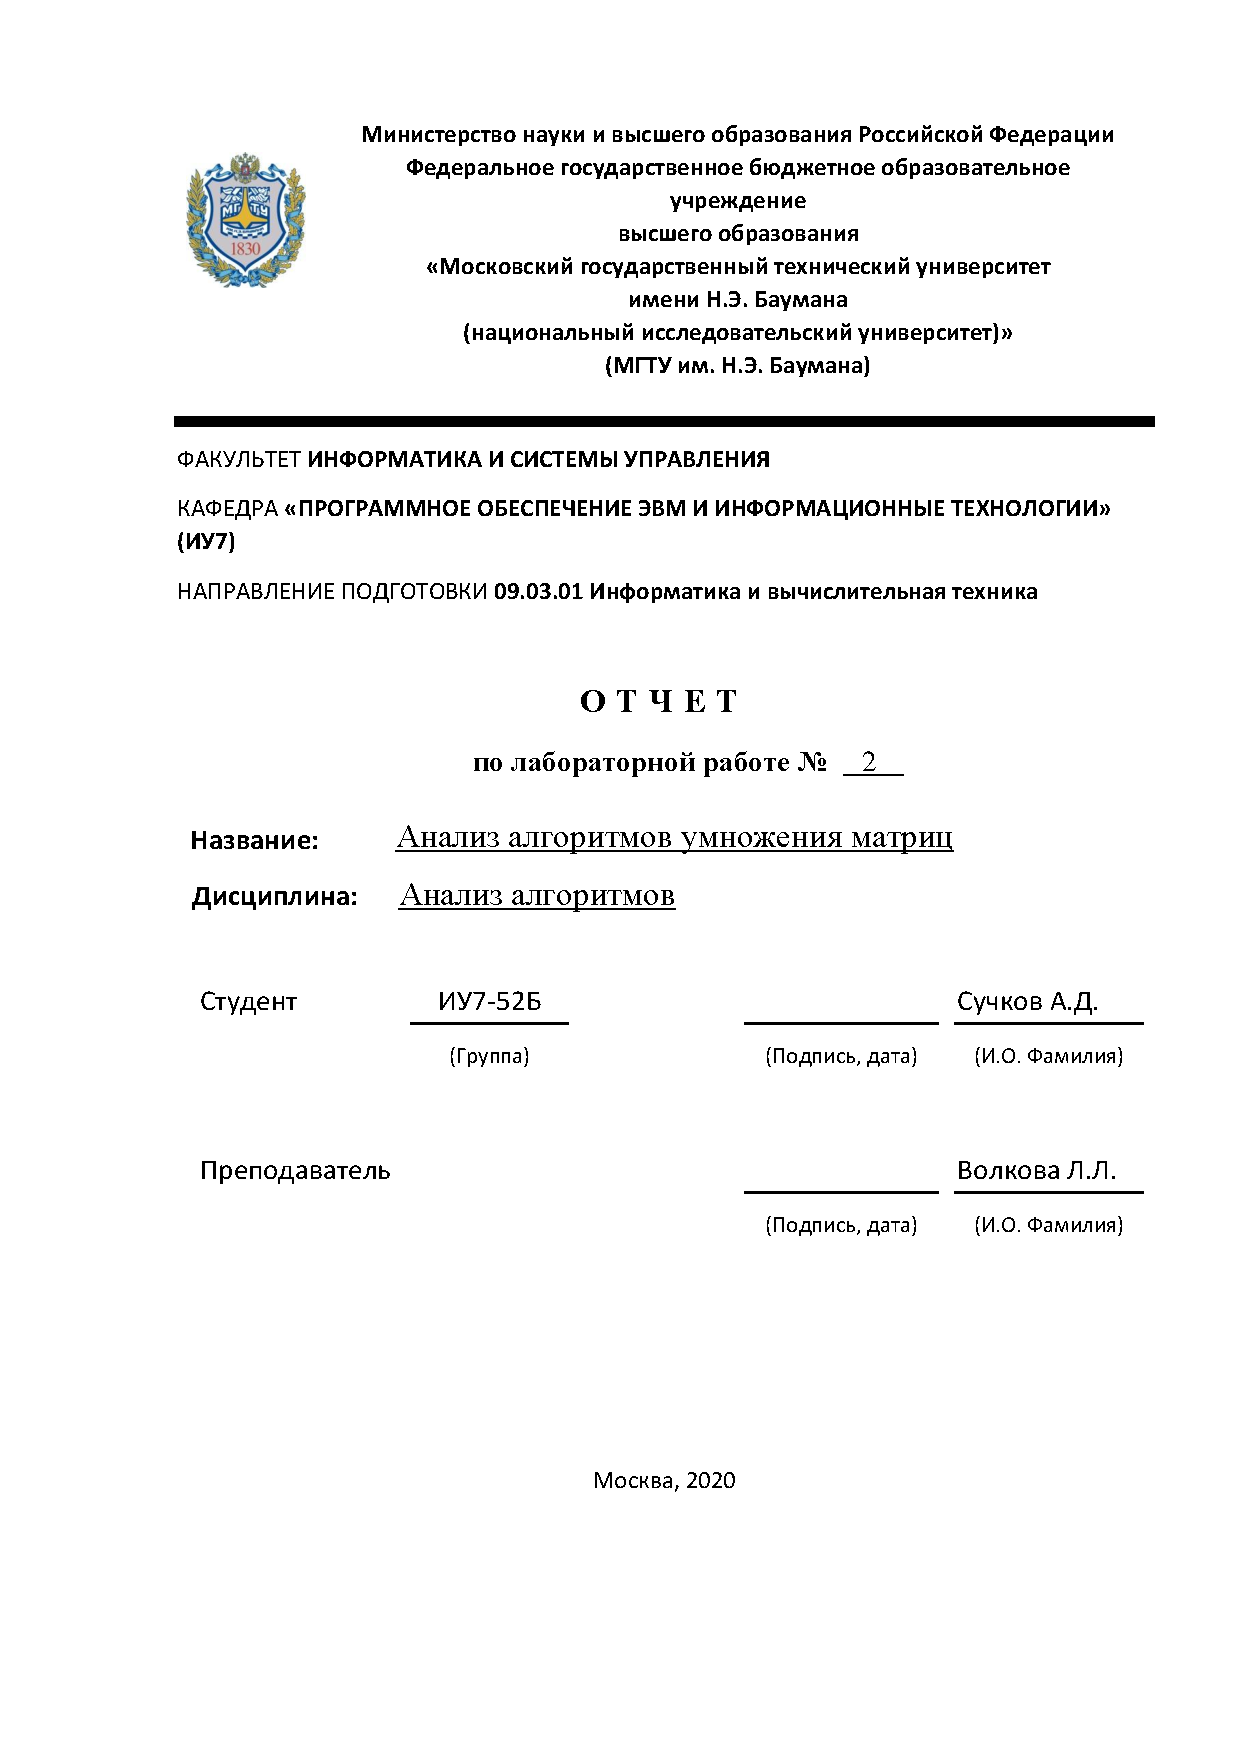
\includepdf[pages=1]{titul.pdf}
% Оглавление
\tableofcontents

\newpage
\chapter*{Введение}
\addcontentsline{toc}{chapter}{Введение}

\textbf{Умножение матриц} - это один из базовых алгоритмов, который широко применяется в различных численных 
методах, и в частности в алгоритмах машинного обучения. 
Многие реализации прямого и обратного распространения сигнала в сверточных слоях неронной сети базируются на 
этой операции. Для перемножения двух матриц необходимо, чтобы количество столбцов в первой матрице совпадало 
с количеством строк во второй. У результирующей матрицы будет столько же строк, сколько в первой матрице, и 
столько же столбцов, сколько во второй. \\ 

Сложность вычисления произведения матриц по определению составляет $O(n^3)$, однако существуют более эффективные 
алгоритмы, которые применяются для больших матриц. 
Вопрос о предельной скорости умножения больших матриц, также как и вопрос о построении наиболее быстрых и усточивых 
практических алгоритмов умножения больших матриц остаётся одной из нерешённых проблем линейной алгебры.

\newpage
\chapter{Аналитическая часть}

Цель данной лабораторной работы заключается в изучении алгоритмов умножения матриц.
Рассматриваются стандартный алгоритм умножения матриц, а также алгоритм Винограда и модифицированный алгоритм 
Винограда.
Требуется рассчитать и изучить затрачиваемое каждым алгоритмом время. \\

В данной лабораторной работе выделено несколько задач:
\begin{itemize}
    \item изучить алгоритмы умножения матриц: стандартный и алгоритм Винограда;
    \item модифицировать алгоритм Винограда;
    \item дать теоретическую оценку базового алгоритма умножения матриц, алгоритму Винограда и модифированному алгоритму Винограда;
    \item реализовать три алгоритма умножения матриц на одном из языков программирования;
    \item сравнить алгоритмы умножения матриц.
\end{itemize}

\section{Стандартный алгоритм умножения матриц}

Пусть даны две матрицы A и B с размерностями $m\times n$ и $n\times l$ соответственно (1.1) и (1.2):

\begin{equation}
    \begin{bmatrix} 
        a_{1,1}      & \textrm{...} & a_{1,n} \\
        \textrm{...} & \textrm{...} & \textrm{...} \\
        a_{m,1}      & \textrm{...} & a_{m,n}
    \end{bmatrix}
\end{equation}

\begin{equation}
    \begin{bmatrix} 
        b_{1,1}      & \textrm{...} & b_{1,l} \\
        \textrm{...} & \textrm{...} & \textrm{...} \\
        b_{n,1}      & \textrm{...} & b_{n,l}
    \end{bmatrix}
\end{equation}

\newpage
В результате умножения, получим матрицу C размерностью $m\times l$ (1.3):

\begin{equation}
    \begin{bmatrix} 
        c_{1,1}      & \textrm{...} & c_{1,l} \\
        \textrm{...} & \textrm{...} & \textrm{...} \\
        c_{m,1}      & \textrm{...} & c_{m,l}
    \end{bmatrix}
\end{equation}

$c_{i,j}=\sum\limits_{r=1}^n a_{i,r} \cdot b_{r,j}$ называется произведением матриц A и B.

\section{Алгоритм Винограда}

Если посмотреть на результат умножения двух матриц, то видно, что каждый элемент в нем представляет 
собой скалярное произведение соответствующих строки и столбца исходных матриц. 
Можно заметить также, что такое умножение допускает предварительную обработку, позволяющую часть работы 
выполнить заранее. \\

Рассмотрим два вектора $V = (v_{1}, v_{2}, v_{3}, v_{4})$ и $W = (w_{1}, w_{2}, w_{3}, w_{4})$. Их 
скалярное произведение (1.4). 
\begin{equation}
    V \cdot W = v_{1} \cdot w_{1} + v_{2} \cdot w_{2} + v_{3} \cdot w_{3} + v_{4} \cdot w_{4}
    \label{formula:1}
\end{equation}

Это равенство можно переписать в виде ()\ref{formula:2})
\begin{equation}
    V \cdot W = (v_{1} + w_{2})(v_{2} + w_{1}) + (v_{3} + w_{4})(v_{4} + w_{3}) - v_{1} \cdot v_{2} - v_{3} \cdot v_{4} - w_{1} \cdot w_{2} - w_{3} \cdot w_{4}
    \label{formula:2}    
\end{equation}

Кажется, что формула \ref{formula:2} задает больше работы, чем первое: вместо четырех умножений мы насчитываем их 
шесть, а вместо трех сложений - десять.
Менее очевидно, что выражение в правой части последнего равенства допускает предварительную обработку: его 
части можно вычислить заранее и запомнить для каждой строки первой матрицы и для каждого столбца второй. 
На практике это означает, что над предварительно обработанными элементами нам придется выполнять лишь первые 
два умножения и последующие пять сложений, а также дополнительно два сложения.

\section{Вывод}

Алгоритм Винограда предлагает подсчитывать значения заранее перед основными вычислениями, что может повысить 
производительность при перемножении достаточно больших матриц. 
Однако с малыми размерами, он может справляться хуже чем другие, но алгоритм можно оптимизировать и добиться 
более высокой скорости подсчёта.

\newpage
\chapter{Конструкторская часть}

\section{Требования к программе}

Для дальнейшего тестирования программы необходимо обеспечить консольный ввод размерностей двух матриц 
и их содержимого, а также обеспечить выбор алгоритма поиска. На выходе должны получить результирующую 
матрицу. Также необходимо реализовать функцию подсчёта процессорного времени, которое могут затрачивать функции.

\section{Схемы алгоритмов}

На рисунках 2.1 - 2.5 приведены схемы алгоритмов умножения матриц.

\begin{figure}[h]
    \center{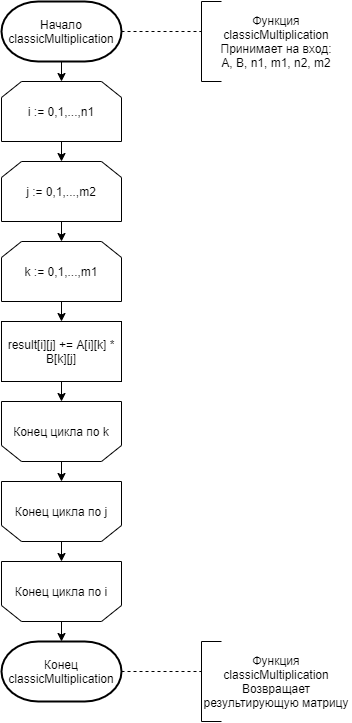
\includegraphics[scale=0.8]{scheme_classic}}
    \caption{Схема стандартного алгоритма умножения матриц}
    \label{fig:image}
\end{figure}

\begin{figure}[h]
    \center{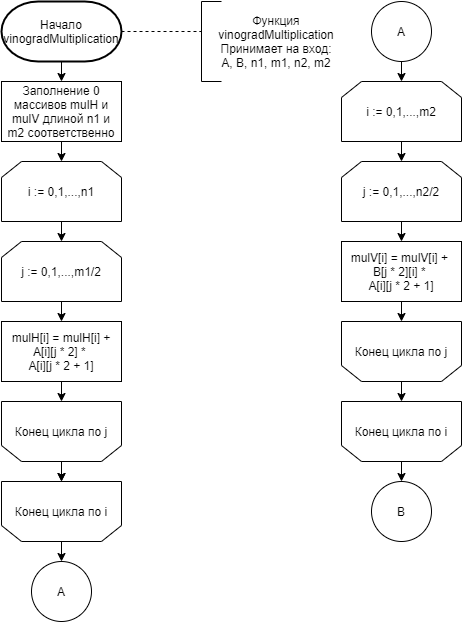
\includegraphics[scale=0.8]{scheme_vinograd_part1}}
    \caption{Схема алгоритма Винограда умножения матриц, часть 1}
    \label{fig:image}
\end{figure}

\begin{figure}[h]
    \center{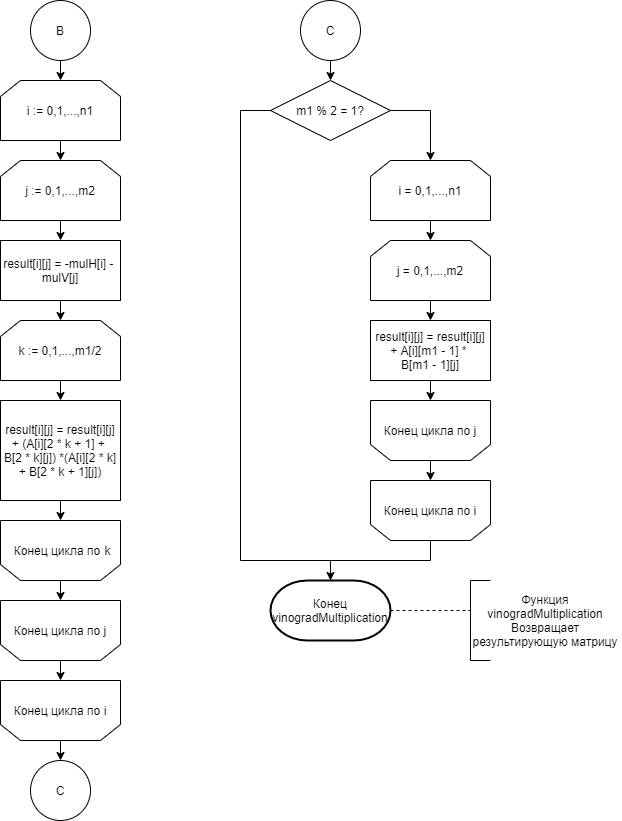
\includegraphics[scale=0.8]{scheme_vinograd_part2}}
    \caption{Схема алгоритма Винограда умножения матриц, часть 2}
    \label{fig:image}
\end{figure} 

\begin{figure}[h]
    \center{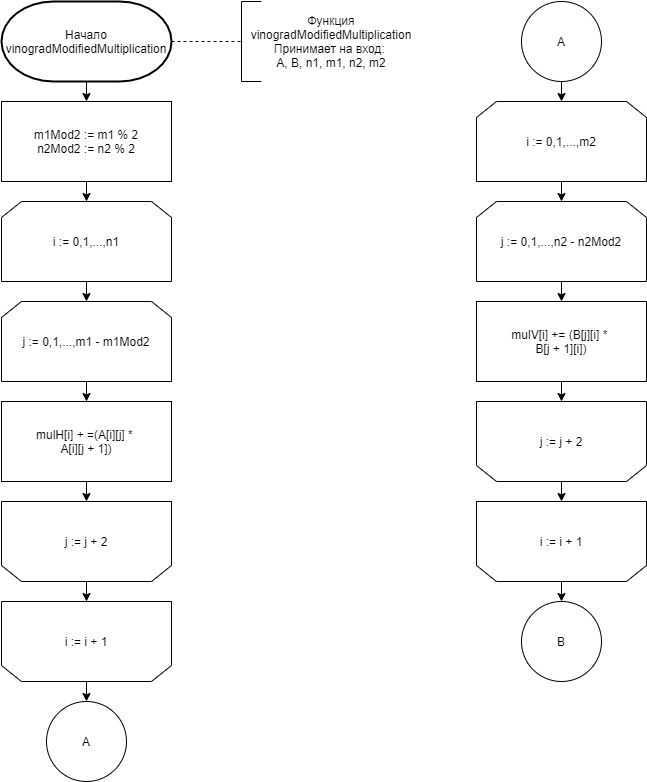
\includegraphics[scale=0.6]{scheme_vinograd_modified_part1}}
    \caption{Схема модифицированного алгоритма Винограда умножения матриц, часть 1}
    \label{fig:image}
\end{figure} 

\begin{figure}[h]
    \center{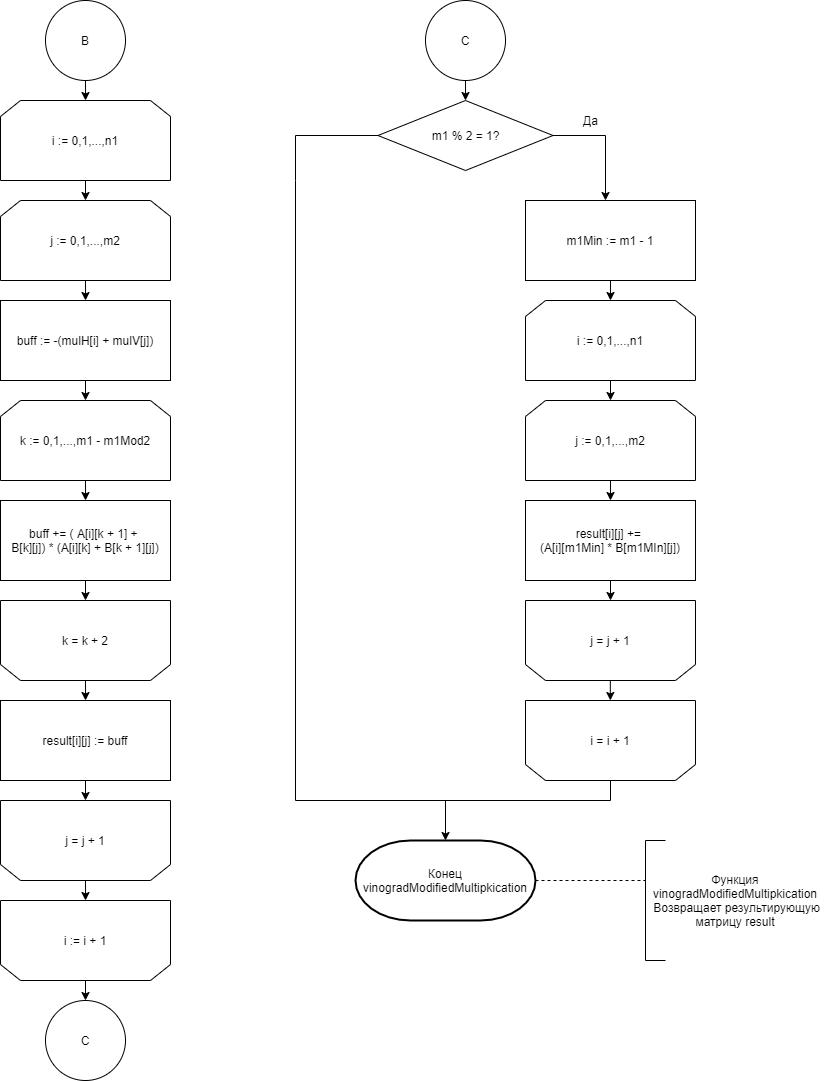
\includegraphics[scale=0.6]{scheme_vinograd_modified_part2}}
    \caption{Схема модифицированного алгоритма Винограда умножения матриц, часть 2}
    \label{fig:image}
\end{figure} 

\section{Подсчёт трудоёмкости алгоритмов}

Для начала оценки алгоритмов, можно ввести специальную модель трудоёмкости:
\begin{itemize}
    \item стоимость базовых операций 1 — +, -, *, /, =, == \dots ;
    \item оценка цикла — $f_{for} = f_{init} + N \cdot (f + f_{body} + f_{post}) + f$, где 
    f - условие цикла, $f_{init}$ - предусловие цикла, $f_{post}$ - постусловие цикла;
    \item стоимость условного перехода примем за 0, стоимость вычисления условия остаётся.
\end{itemize}

\textbf{Для стандартного алгоритма умножения} с матрицами A и B и размерами $n\times m$ и $m\times l$ 
соответственно: \\

$f = 2 + n \cdot (2 + 2 + l \cdot (2 + 2 + m \cdot (2 + 6 + 2))) = 10nlm + 4ln  + 4n + 2$ \\

\textbf{Для алгоритма Винограда} при тех же матрицах и их размерах. \\

Для более понятного подсчёта, можно составить таблицу (таблица 2.1), а затем подсчитать общую трудоёмкость:

\begin{displaymath}
    f = 13mnl + 7.5mn + 7.5lm + 11ln + 8n + 4l + 14 + \left \{ 
    \begin{array}{ll}  
        0, \textrm{если m чётное} \\ 
        15 \cdot l \cdot n + 4 \cdot n + 2, \textrm{иначе} 
    \end{array} \right.
\end{displaymath}

\begin{table}[h]
\caption{трудоёмкость алгоритма Винограда}  
\label{tabular:timesandtenses}
\begin{center}
\begin{tabular}{ | l | l | }
\hline
    Часть алгоритма            & Трудоёмкость                                                        \\ \hline
    Инициализация mulH и mulV  & $2 \cdot 3$                                                         \\ \hline
    Заполнение mulH            & $2 + n \cdot (2 + 2 + m / 2 \cdot (3 + 6 + 6))$                     \\ \hline
    Заполнение mulV            & $2 + l \cdot (2 + 2 + m / 2 \cdot (3 + 6 + 6))$                     \\ \hline
    Подсчёт результата         & $2 + n \cdot (2 + 2 + l \cdot (2 + 7 + 2 + m / 2 \cdot (3 + 23)))$  \\ \hline
    Условный оператор нечёт. m & $2$                                                                 \\ \hline
    Для матриц с нечёт m       & $2 + n \cdot (2 + 2 + l \cdot (2 + 8 + 5))$                         \\ \hline
\end{tabular}
\end{center}
\end{table}

\textbf{Для оптимизированного алгоритма Винограда} при тех же матрицах и размерах. 
Для более понятного подсчёта, можно тоже составить таблицу (таблица 2.2).

\begin{displaymath}
    f = 8mnl + 5mn + 5lm + 12ln + 8n + 4l + 18 + \left \{ 
    \begin{array}{ll}  
        0, \textrm{если m чётное} \\ 
        10 \cdot l \cdot n + 4 \cdot n + 4, \textrm{иначе} 
    \end{array} \right.
\end{displaymath}

\begin{table}[h]
\caption{трудоёмкость оптимизированного алгоритма Винограда}  
\label{tabular:timesandtenses}
\begin{center}
\begin{tabular}{ | l | l | }
\hline
        Часть алгоритма               & Трудоёмкость                                                            \\ \hline
        Инициализация mulH и mulV     & $2 \cdot 3$                                                             \\ \hline
        Инициализация m1Mod2          & $2 \cdot 2$                                                             \\
        и n2Mod2                      &                                                                         \\ \hline
        Заполнение mulH               & $2 + n \cdot (2 + 2 + m / 2 \cdot (2 + 5 + 3))$                         \\ \hline
        Заполнение mulV               & $2 + l \cdot (2 + 2 + m / 2 \cdot (2 + 5 + 3))$                         \\ \hline
        Подсчёт результата            & $2 + n \cdot (2 + 2 + l \cdot (2 + 5 + 3 + 2 + $                        \\
                                      & $ + m / 2 \cdot (2 + 14)))$                                             \\ \hline
        Условный оператор нечёт. m    & $2$                                                                     \\ \hline
        Для матриц с нечёт m          & $2 + 2 + n \cdot (2 + 2 + l \cdot (2 + 6 + 2))$                         \\ \hline
\end{tabular}
\end{center}
\end{table}

\section{Вывод}

Были составлены схемы и подсчитана трудоёмкость для каждого алгоритма.
Из последнего можно увидеть, что оптимизированный алгоритм Винограда менее трудоёмкий, чем неоптимизированный. 

\newpage
\chapter{Технологическая часть}

\section{Выбор языка программирования}

В качестве языка программирования было решено выбрать Python 3, так как уже имеется опыт работы с 
библиотеками и инструмантами языка, которые позволяют реализовать и провести исследования над 
умножением матриц.

\section{Реализации алгоритмов}

В листингах 3.1 - 3.3 приведены реализации алгоритмов умножения на Python.

\textrm{Листинг 3.1: классический алгоритм умножения матриц}
\begin{lstlisting}[frame=single, numbers=left]
def classicMultiplication(A, B, isPrint):
    result = [[0 for j in range(len(A))] 
                 for i in range(len(B[0]))]

    for i in range(len(A)):
        for j in range(len(B[0])):
            for k in range(len(A[i])):
                result[i][j] += A[i][k] * B[k][j]
    
    if (isPrint):
        print("\n>>> Result with classic method:")
        printMatrix(result)
\end{lstlisting}

\textrm{Листинг 3.2: алгоритм умножения матриц Винограда}
\begin{lstlisting}[frame=single, numbers=left]
def vinogradMultiplication(A, B, isPrint):
    n1, m1 = len(A), len(A[0])
    n2, m2 = len(B), len(B[0])

    mulH = [0 for _ in range(n1)]
    mulV = [0 for _ in range(m2)]

    result = [[0 for j in range(n1)] for i in range(m2)]

    for i in range(n1):
        for j in range(int(m1 / 2)):
            mulH[i] = mulH[i] + A[i][j * 2] * 
                                A[i][j * 2 + 1]
        
    for i in range(m2):
        for j in range(int(n2 / 2)):
            mulV[i] = mulV[i] + B[j * 2][i] * 
                                B[j * 2 + 1][i]

    for i in range(n1):
        for j in range(m2):
            result[i][j] = -mulH[i] - mulV[j]

            for k in range(int(m1 / 2)):
                result[i][j] = result[i][j] + 
                    ((A[i][2 * k + 1] + B[2 * k][j]) * 
                     (A[i][2 * k] + B[2 * k + 1][j]))
    
    if (m1 % 2):
        for i in range(n1):
            for j in range(m2):
                result[i][j] = result[i][j] + 
                (A[i][m1 - 1] * B[m1 - 1][j])
    
    if (isPrint):
        print("\n>>> Result with vinograd method:")
        printMatrix(result)
\end{lstlisting}

\textrm{Листинг 3.3: оптимизированный алгоритм Винограда}
\begin{lstlisting}[frame=single, numbers=left]
def vinogradMultiplicationModified(A, B, isPrint):
    n1, m1 = len(A), len(A[0])
    n2, m2 = len(B), len(B[0])

    mulH = [0 for _ in range(n1)]
    mulV = [0 for _ in range(m2)]

    result = [[0 for j in range(n1)] 
                 for i in range(m2)]

    m1Mod2 = m1 % 2
    n2Mod2 = n2 % 2

    for i in range(n1):
        for j in range(0, m1 - m1Mod2, 2):
            mulH[i] += A[i][j] * A[i][j + 1]
    
    for i in range(m2):
        for j in range(0, n2 - n2Mod2, 2):
            mulV[i] += B[j][i] * B[j + 1][i]
    
    for i in range(n1):
        for j in range(m2):
            buff = -(mulH[i] + mulV[j])

            for k in range(0, m1 - m1Mod2, 2):
                buff += ((A[i][k + 1] + B[k][j]) * 
                         (A[i][k] + B[k + 1][j]))
            result[i][j] = buff
    
    if m1Mod2:
        m1Min = m1 - 1
        for i in range(n1):
            for j in range(m2):
                result[i][j] += A[i][m1Min] * B[m1Min][j]
    if isPrint:
        print("\nResult with modified vinograd method:")
        printMatrix(result)
\end{lstlisting}

\section{Оптимизация алгоритма Винограда}

Для оптимизации алгоритма были внесены некоторые изменения. \\

Заранее высчитываются значения, для избавления от деления в цикле. См. листинг 3.4.

\textrm{Листинг 3.4: избавление от деления в цикле}
\begin{lstlisting}[frame=single, numbers=left]
def vinogradMultiplicationModified(A, B, isPrint):
    ...

    m1Mod2 = m1 % 2
    n2Mod2 = n2 % 2

    for i in range(n1):
        for j in range(0, m1 - m1Mod2, 2):
            mulH[i] += A[i][j] * A[i][j + 1]
    
    for i in range(m2):
        for j in range(0, n2 - n2Mod2, 2):
            mulV[i] += B[j][i] * B[j + 1][i]
    
    ...
\end{lstlisting}

Заменяется обычное сложение (mulV[i] = mulV[i] + ...) на более оптимизированный вариант (mulV[i] += ..., аналогично 
и в других подобных местах). См. листинг 3.5.

\textrm{Листинг 3.5: оптимизация сложения}
\begin{lstlisting}[frame=single, numbers=left]
def vinogradMultiplicationModified(A, B, isPrint):
    ...

    for i in range(n1):
        for j in range(0, m1 - m1Mod2, 2):
            mulH[i] += A[i][j] * A[i][j + 1]


    for i in range(m2):
        for j in range(0, n2 - n2Mod2, 2):
            mulV[i] += B[j][i] * B[j + 1][i]

    for i in range(n1):
        for j in range(m2):
            buff = -(mulH[i] + mulV[j])

            for k in range(0, m1 - m1Mod2, 2):
                buff += ((A[i][k + 1] + B[k][j]) * 
                         (A[i][k] + B[k + 1][j]))

            result[i][j] = buff
    
    if m1Mod2:
        m1Min = m1 - 1
        
        for i in range(n1):
            for j in range(m2):
                result[i][j] += A[i][m1Min] * B[m1Min][j]

    ...
\end{lstlisting}

Инициализируется специальный буфер для накопления результата умножения, который позже сбрасывается 
в ячейку матрицы. См. листинг 3.6.

\textrm{Листинг 3.6: оптимизация, при помощи буфера}
\begin{lstlisting}[frame=single, numbers=left]
def vinogradMultiplicationModified(A, B, isPrint):
    ...

    for i in range(n1):
        for j in range(m2):
            buff = -(mulH[i] + mulV[j])

            for k in range(0, m1 - m1Mod2, 2):
                buff += ((A[i][k + 1] + B[k][j]) * 
                         (A[i][k] + B[k + 1][j]))

            result[i][j] = buff

    ...
\end{lstlisting}

\section{Оценка затрачиваемого времени}

Для замера процессорного времени выполнения алгоритмов используется библиотека time \cite{time_bib}. 
В листинге 3.7 приведена функция наполнения случайными числами матрицы с заданным размером. 
В листинге 3.8 приведены функции с помощью которых производятся замеры времени. \\

\textrm{Листинг 3.7: наполнение матрицы случайными числами}
\begin{lstlisting}[frame=single, numbers=left]
def generateMatrix(size):
    return [[random.randint(0, 9) for _ in range(size)] 
                                  for _ in range(size)]
\end{lstlisting}

\textrm{Листинг 3.8: функции для замера времени}
\begin{lstlisting}[frame=single, numbers=left]
def doTimeTest(method, A, B):
    t1 = process_time()
    method(A, B, False)
    t2 = process_time()

    return t2 - t1

def multiplicationTimeTest():
    sizesMod2 = [100, 150, 200]
    sizesNotMod2 = [101, 151, 201]

    for size in sizesMod2:
        A = generateMatrix(size)
        B = generateMatrix(size)

        print(">>> For classic with       len = ", size, 
        "Time:", doTimeTest(classicMultiplication, A, B))
        
        print(">>> For Vinograd with      len = ", size, 
        "Time:", doTimeTest(vinogradMultiplication, A, B))
        
        print(">>> For Vinograd mod. with len = ", size, 
        "Time:", doTimeTest(vinogradMultiplicationModified, 
                            A, B))

    for size in sizesNotMod2:
        A = generateMatrix(size)
        B = generateMatrix(size)

        print(">>> For classic with       len = ", size, 
        "Time:", doTimeTest(classicMultiplication, A, B))
        
        print(">>> For Vinograd with      len = ", size, 
        "Time:", doTimeTest(vinogradMultiplication, A, B))
        
        print(">>> For Vinograd mod. with len = ", size, 
        "Time:", doTimeTest(vinogradMultiplicationModified, 
                            A, B))
\end{lstlisting}

\section{Вывод}

Были реализованы функции алгоритмов перемножения матриц на языке Python 3, а также функции тестирования 
и подсчёта процессорного времени. 

\newpage
\chapter{Исследовательская часть}

Измерения процессорного времени проводятся при одинаковых размерах матриц и при этом тестируются как чётные 
размеры, так и нечётные: 100, 101, 150, 151, 200, 201. 

\section{Результаты экспериментов}

Проведя измерения процессорного времени выполнения реализованных алгоритмов, можно составить для чётных размеров 
таблицу 4.1 и для нечётных таблицу 4.2.

\begin{table}[h]
\caption{Результаты замеров процессорного времени в секундах, для чётных размеров}
\label{tabular:timesandtenses}
\begin{center}
\begin{tabular}{ | l | l | l | l | }
\hline
    Название метода $\backslash$ Размер & 100   & 150   & 200   \\ \hline
    Стандартный                         & 0.421 & 1.578 & 3.406 \\ \hline
    алгоритм Винограда                  & 0.453 & 1.563 & 3.625 \\ \hline
    оптимизированный алг. Винограда     & 0.328 & 0.969 & 2.422 \\ \hline
\end{tabular}
\end{center}
\end{table}

\begin{table}[h]
\caption{Результаты замеров процессорного времени в секундах, для нечётных размеров}
\label{tabular:timesandtenses}
\begin{center}
\begin{tabular}{ | l | l | l | l | }
\hline
        Название метода $\backslash$ Размер & 101   & 151   & 201   \\ \hline
        Стандартный                         & 0.391 & 1.469 & 3.422 \\ \hline
        алгоритм Винограда                  & 0.516 & 1.813 & 3.813 \\ \hline
        оптимизированный алг. Винограда     & 0.313 & 1.125 & 2.766 \\ \hline
\end{tabular}
\end{center}
\end{table}

\section{Вывод}

Анализируя результаты замеров затрачиваемого времени и тестируя алгоиртмы на разных размерах, 
можно сказать, что стандартный алгоритм умножения матриц выигрывает по времени у остальных, но на малых 
размерах, однако его главным преимущестом является стабильность, то есть алгоритм не зависит от чётности 
размера матрицы. \\

Также стоит заметить, что модифицированный алгоритм Винограда показывает наилучшее время на средних размерах, в то 
время, как неоптимизированный алгоритм Винограда показывает наихудшее. 
В неоптимизированномалгоритме Винограда приходится неоднократно вычислять одни и те же значения, что может замедлять 
его.

\newpage
\chapter*{Заключение}
\addcontentsline{toc}{chapter}{Заключение}

В ходе работы были изучены алгоритмы умножения матриц. 
Реализованы 3 алгоритма, приведен программный код реализации алгоритмов по умножению матриц.
Была подсчитана трудоемкость каждого из алгоритмов. 
А также было проведено сравнение алгоритмов по времени и трудоемкости.\\

Цель работы достигнута. 
Получены практические навыки реализации алгоритмов Винограда и стандартного алгоритма, а также проведена 
исследовательская работа по оптимизации и вычислении трудоемкости алгоритмов.



\newpage
\renewcommand\bibname{Список литературы}
\addcontentsline{toc}{chapter}{Список литературы}
\makeatletter % список литературы
\def\@biblabel#1{#1. }
\makeatother
\begin{thebibliography}{2}
    \bibitem{analyse_info} Дж. Макконнел. Анализ алгоритмов. Активный обучающий подход. -- М.: Техносфера, 2017. -- 267с.
    \bibitem{time_bib} Документация на официальном сайте Python про библиотеку time [Электронный ресурс]. Режим доступа: https://docs.python.org/3/library/time.html (дата обращения 23.09.2020)
\end{thebibliography}

\end{document}

